% CVPR 2027 submission: main paper. Ported from ../iclr/main.tex (frozen reference).
% Kit: author-kit-CVPR2027-v1-latex.zip (cvpr.sty "2027 LaTeX class for IEEE CVPR").
% Build: `make` (draft) or `make submit` (fails on any leftover \TODO/\com).

\documentclass[10pt,twocolumn,letterpaper]{article}

%%%%%%%%% PAPER TYPE
% \usepackage{cvpr}              % CAMERA-READY
\usepackage[review]{cvpr}      % REVIEW version
% \usepackage[pagenumbers]{cvpr} % arXiv

%% Shared preamble for main.tex and supp.tex (CVPR 2027 kit).
%% Loaded by both documents BEFORE hyperref (the kit loads hyperref after this).
%% cvpr.sty already provides: times, xspace, xcolor[dvipsnames], graphicx,
%% amsmath, amssymb, booktabs, natbib[numbers], caption, subcaption, url,
%% enumitem, and (at end of preamble) cleveref.

\usepackage{amsthm}
\newtheorem{lemma}{Lemma}
\usepackage{multirow}
\usepackage{csquotes}   % \enquote{...}
\usepackage{xr-hyper}   % cross-document refs main <-> supp; must precede hyperref

% A little slack for lines TeX cannot break well (long \texttt identifiers).
\emergencystretch=1.5em

% Float packing (standard loosenings; no kit layout rule is changed).
\renewcommand{\topfraction}{0.92}
\renewcommand{\bottomfraction}{0.75}
\renewcommand{\textfraction}{0.07}
\renewcommand{\floatpagefraction}{0.80}
\renewcommand{\dbltopfraction}{0.92}
\renewcommand{\dblfloatpagefraction}{0.80}
\setcounter{topnumber}{3}
\setcounter{bottomnumber}{2}
\setcounter{totalnumber}{4}
\setcounter{dbltopnumber}{2}

% ---------------------------------------------------------------------------
% Draft switch. Default build = draft: \TODO, \UNMEASURED and \com render in
% colour. Submission build (`make submit`, which defines \submission) turns
% draft off, and then every leftover \TODO / \UNMEASURED / \com is a hard error.
% ---------------------------------------------------------------------------
\newif\ifdraft\drafttrue
\ifdefined\submission\draftfalse\fi
\ifdraft
  \newcommand{\TODO}[1]{\textcolor{red}{\textbf{[TODO: #1]}}}
  \newcommand{\UNMEASURED}[1]{\textcolor{red}{\textbf{[UNMEASURED: #1]}}}
  \newcommand{\com}[1]{\textcolor{blue}{Comment: #1}}
\else
  \newcommand{\TODO}[1]{\PackageError{paper}{Unresolved TODO: #1}{}}
  \newcommand{\UNMEASURED}[1]{\PackageError{paper}{Unmeasured claim: #1}{}}
  \newcommand{\com}[1]{\PackageError{paper}{Unaddressed comment: #1}{}}
\fi

% ---------------------------------------------------------------------------
% Cross-document references. The supplementary is a separate PDF; labels are
% imported with xr-hyper under a prefix (main imports supp as S-*, supp imports
% main as M-*; the prefix also keeps the two bibliographies' numbers apart).
% Always go through these macros, never \ref{S-...} by hand.
%   main  -> supp : \suppsec \suppfig \supptab
%   supp  -> main : \mainsec \mainfig \maintab \maineq
% ---------------------------------------------------------------------------
\newcommand{\suppsec}[1]{Supp.~Sec.~\ref{S-#1}}
\newcommand{\suppfig}[1]{Supp.~Fig.~\ref{S-#1}}
\newcommand{\supptab}[1]{Supp.~Tab.~\ref{S-#1}}
\newcommand{\mainsec}[1]{main paper \S\ref{M-#1}}
\newcommand{\mainfig}[1]{main paper Fig.~\ref{M-#1}}
\newcommand{\maintab}[1]{main paper Tab.~\ref{M-#1}}
\newcommand{\maineq}[1]{main paper Eq.~\ref{M-#1}}

% ---------------------------------------------------------------------------
% Names (ported from iclr/main.tex). Every name in \mbox so it never breaks at
% its internal hyphen; arms/probes/baselines in \textsc, metrics roman.
% ---------------------------------------------------------------------------
% -- the two realism metrics
\newcommand{\mvkid}{\mbox{MV-KID}}      % multi-view render KID (DINOv2, 4 views)
\newcommand{\vkid}{\mbox{V-KID}}        % voxel-descriptor KID
\newcommand{\blockscore}{\mbox{BlockScore}}

% -- probes (real data, corrupted in a known way)
\newcommand{\solidify}{\mbox{\textsc{Fill-Interior}}}
\newcommand{\matshuffle}{\mbox{\textsc{Material-Shuffle}}}
\newcommand{\monochrome}{\mbox{\textsc{Monochrome}}}
\newcommand{\singlemode}{\mbox{\textsc{Single-Mode}}}
\newcommand{\traincopy}{\mbox{\textsc{Train-Copy}}}
\newcommand{\realheld}{\mbox{\textsc{Real}}}
\newcommand{\hollow}{\mbox{\textsc{Hollow-Shell}}}
\newcommand{\growshell}{\mbox{\textsc{Grow-Shell}}}

% -- procedural baselines
\newcommand{\patchstitch}{\mbox{\textsc{Patch-Stitch}}}
\newcommand{\gabled}{\mbox{\textsc{Gabled-House}}}
\newcommand{\hollowbox}{\mbox{\textsc{Hollow-Box}}}
\newcommand{\randomvox}{\mbox{\textsc{Random-Voxels}}}
\newcommand{\copynoise}{\mbox{\textsc{Train-Copy+Noise}}}

% -- generative arms
\newcommand{\voxar}{\mbox{\textsc{Voxel-AR}}}
\newcommand{\voxarun}{\mbox{\textsc{Voxel-AR-U}}}
\newcommand{\llmft}{\mbox{\textsc{LLM-FT}}}
\newcommand{\llmgeo}{\mbox{\textsc{LLM-FT-Geo}}}


\definecolor{cvprblue}{rgb}{0.21,0.49,0.74}
\usepackage[pagebackref,breaklinks,colorlinks,allcolors=cvprblue]{hyperref}

% Supplementary labels (app:*, fig:pipeline, tab:seven, ...) come from supp.aux.
% Build supp once before main (the Makefile does this).
\externaldocument[S-]{supp}

\def\confName{CVPR}
\def\confYear{2027}
% The 2027 kit removed the Paper ID from the review header (kit README:
% "removed the Paper ID to reduce the risk of leaking IDs"). Kept here only as a
% placeholder for bookkeeping; cvpr.sty does not print it.
\def\paperID{*****}

%%%%%%%%% TITLE
\title{A Building Is Not Its Silhouette: Structural Blindness in 3D Generation Evaluation}

%%%%%%%%% AUTHORS (review mode prints "Anonymous CVPR submission" regardless)
\author{Anonymous CVPR submission}

\begin{document}

% Title plus full-width teaser on page 1.
\twocolumn[{%
\renewcommand\twocolumn[1][]{#1}%
\maketitle
% Full-width teaser under the title. Input by main.tex inside \twocolumn[...] so it lands on page 1.
% Textured renders differ by ~0.8/255 (atlas repacking); bit-identity holds under flat colours only.
\begin{center}
  \centering
  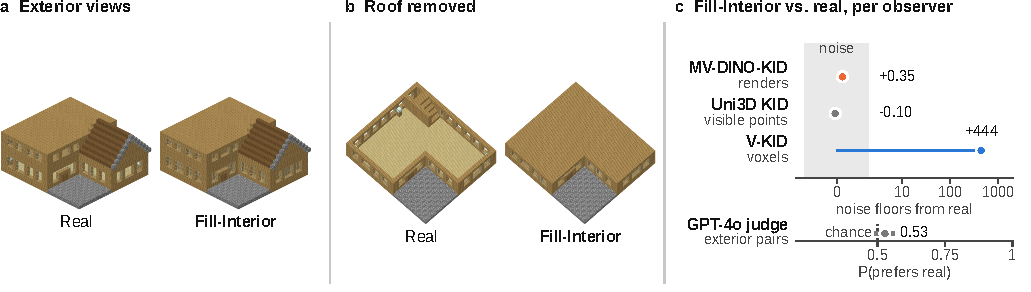
\includegraphics[width=\textwidth]{figures/fig1_teaser}
  \captionsetup{type=figure}
  \caption{\textbf{A metric ranks only what it observes.}
  \textbf{(a)}~A real held-out house and its \solidify{} copy, in which every sealed
  room is filled with the house's own material ($+138\%$ blocks on this build; median
  $+33\%$ over $200$ held-out houses). Rendered in flat colours, the four metric views of this
  build are bit-identical to those of its copy.
  \textbf{(b)}~With the roof removed, the real house has rooms and the copy is solid.
  \textbf{(c)}~Distance of the filled corpus from real data under each observer, in
  noise floors (the shaded band is $\pm 2$). The multi-view DINOv2 KID on exterior
  renders and Uni3D on visible-surface points ($n{=}128$; seeds $-0.1$ and $+0.4$) stay
  inside the noise, and a GPT-4o judge shown exterior pairs prefers the real house in
  $0.53$ of trials ($95\%$ CI $[0.50, 0.56]$). \vkid{} on voxels places the same corpus
  $444$ noise floors away. The render and voxel values come from the $n{=}256$
  leaderboard (\S\ref{sec:complementary}); published builds come from 3D-Craft
  (\suppsec{app:data}).}
  \label{fig:teaser}
\end{center}

\vspace{0.5em}
}]

% Active abstract: version A of STRUCTURE_ABSTRACT.md (user decision 2026-11-04).
% Headline numbers are from the n=256 leaderboard of record
% (run_20261103_090315_bench_n_256_leaderboard_of_record): 0.35 and 444.36.
% "Five image encoders" = DINOv2-B plus the four others of Supp. Tab. tab:ablation.
% Older drafts are kept commented below for reference.
\begin{abstract}
Generative models of 3D structure are ranked by metrics that observe only part of what they score: rendered exterior views, points sampled from visible surfaces, or a judge shown images. A metric cannot rank what its observations discard, and for buildings, LEGO models and indoor scenes the discarded part is often the interior, which decides whether a structure can be entered, assembled or navigated. We make this limit measurable with complement probes that alter a structure while keeping every exterior-visible face identical. Filling the sealed rooms of real Minecraft houses adds a median 33\% more blocks, yet a multi-view DINOv2 kernel distance places the filled corpus 0.35 noise floors (units of the metric's own real-versus-real sampling spread) from real data, in the same significance group. The blindness holds for seven render statistics, five image encoders and up to sixteen views, for Uni3D and ULIP-2 point-cloud encoders and Chamfer and earth mover's distances on visible-surface points, and for a GPT-4o judge, across Minecraft, LEGO and Objaverse meshes. Changing only the observation, by cutting the views open or sampling interior faces, recovers the signal. We introduce V-KID, a CPU-only voxel metric that separates the probe by 444 noise floors and is blind exactly where render metrics see, and a protocol that admits a metric to a leaderboard only after it passes gates on ordering, invariance and sample-size stability, which Fr\'echet distance fails. Applied to the published generator BrickGPT, the protocol finds a geometric gap 2.2 times its render gap in effect size.
\end{abstract}

% Previous active draft (2026-11-02, 0925 protocol numbers 0.14 / 202):
% \begin{abstract}
% Generative models of 3D structure are evaluated by rendering a few exterior views, embedding them with a pretrained encoder, and measuring a distribution distance to real data. This protocol cannot see whether a structure has an inside, yet interiors are what make a building walkable, a LEGO model buildable, and a game asset usable. We measure the gap with a controlled corruption: filling every sealed room of real Minecraft buildings with their own material adds a median 33\% more blocks and leaves the silhouette unchanged. A DINOv2 kernel distance on four views moves 0.14 noise floors, inside the spread of real data, while a kernel distance on voxel descriptors moves 202. Seven render-space statistics, five encoders, up to sixteen views and a LEGO corpus all miss the corruption, while resolving every corruption that reaches the exterior. Cutaway views recover it with the same encoder, placing the failure in the view protocol, and under opaque rendering we prove no exterior-view metric can detect it. We therefore introduce V-KID, a CPU-only geometric metric with the complementary blind spot, and a validation protocol that admits a metric to a leaderboard only after it passes gates on ordering, invariance and sample-size stability. Fr\'echet distance and the biased MMD fail these gates.
% \end{abstract}

% \begin{abstract}
% Many existing evaluation protocols for 3D generative models assess realism by rendering generated structures from a limited set of viewpoints and comparing pretrained visual features of these renderings against those of real data. While effective for measuring visual similarity and distributional realism, such protocols provide limited guarantees about properties that are intrinsically three-dimensional or functional. In particular, exterior-view evaluation may fail to detect missing or incoherent interior geometry, inaccessible spaces, collisions, or invalid spatial layouts. For structures intended to be inhabited, assembled, or navigated—such as Minecraft buildings, LEGO models, or game environments—these properties are central to usability rather than merely appearance.   We measure this failure with a controlled corruption. Filling every sealed void in a corpus of real buildings adds a median of $33\%$ more blocks and leaves the exterior silhouette untouched. A multi-view DINOv2 kernel distance places the corrupted corpus at just $0.38$ noise floors from real data, while our proposed geometric metric on voxel descriptors (V-KID) successfully separates it by over $200$ noise floors. Seven render-space statistics, five encoders, view budgets up to sixteen views, and a second domain all miss this corruption while resolving every other one we apply. Under an opaque renderer, filling sealed voids cannot change any exterior view, meaning no exterior-view statistic can separate it at any sample size.   To close this blind spot, we introduce a validation protocol that requires metrics to pass strict gates for monotonicity, invariance, and sample-size stability before they can rank models. Measuring geometry directly alongside renders provides a complete evaluation. Applying this protocol to our own models demonstrated its practical necessity by exposing an $87\%$ train-test contamination in a generator we had treated as a top result, proving the danger of deploying unvalidated metrics.
% \end{abstract}

% \begin{abstract}
% %TL;DR of paragraph: the field renders exterior views to evaluate 3D structure, and that protocol cannot see interiors, which is the property that makes a structure usable.
% Many existing evaluation protocols for 3D generative models assess realism by rendering generated structures from a limited set of viewpoints and comparing pretrained visual features of these renderings against those of real data. While effective for measuring visual similarity and distributional realism, such protocols provide limited guarantees about properties that are intrinsically three-dimensional or functional. In particular, exterior-view evaluation may fail to detect missing or incoherent interior geometry, inaccessible spaces, collisions, or invalid spatial layouts. For structures intended to be inhabited, assembled, or navigated—such as Minecraft buildings, LEGO models, or game environments--these properties are central to usability rather than merely appearance.

% % Generative models of discrete {3D} structure are evaluated by rendering a few
% % exterior views, embedding them with a pretrained encoder, and measuring a
% % distribution distance to real data. This protocol cannot see whether a structure
% % has an inside. Interior layout is what makes a generated structure usable rather than decorative: a Minecraft build someone walks through, a LEGO model someone assembles, a game asset that needs navigable space and collision volumes.

% %TL;DR of paragraph: the measurement, its scope across statistics and encoders, and the impossibility result that explains it.
% We measure the failure with a controlled corruption. Filling every sealed void in
% a corpus of real buildings adds a median of $33\%$ more blocks and leaves the
% exterior silhouette untouched. A multi-view DINOv2 kernel distance places the
% corrupted corpus $0.38$ \com{what does that number mean? Should we immediately know what these mean? There is not really a baseline to give them meaning?} of its own sampling noise from real data, while a kernel
% distance on voxel descriptors places it beyond $200$. Seven render-space
% statistics, five encoders, view budgets up to sixteen views, and a second domain
% all miss this corruption while resolving every other one we apply. Cutaway views
% recover the signal with the same encoder and the same statistic, which locates
% the failure in the view protocol rather than in the features. Under an opaque
% renderer the invisibility is exact: filling sealed voids cannot change any
% exterior view, so no encoder and no statistic can separate it at any sample size.

% %TL;DR of paragraph: the prescription is to validate a metric before ranking with it, and applying it cost us our own headline result.
% \com{We might want to word it as we introduce this because it makes it seem like our only contribution is noticing the problem, not giving a potential solution} We therefore require a metric to pass a validation protocol before it ranks
% models. Candidates are scored against corruptions of known severity and must
% satisfy monotonicity, invariance, and sample-size stability, with separate
% disqualification gates for memorization and mode collapse. Measuring geometry
% directly alongside the renders closes the blind spot. Applying the protocol to
% our own models \com{What? Why talk about this? This just makes it seems like we were just dumb and didn't use splits well enough} exposed $87\%$ train-test contamination in the generator we had
% treated as this project's best result, which lost its advantage over the
% baselines once retrained on a clean split.
% \end{abstract}

\section{Introduction}

%TL;DR of paragraph: interiors are why a generated building is useful, and no exterior view shows them.
Many of us are taught at a young age that we shouldn't judge a book by its cover. A building can be examined the same way. It may have rooms, doors--an interior. And, in many cases, structures rely on these interior layouts to make them usable rather than decorative. Consider a Minecraft build someone walks through, a LEGO model someone assembles, or an indoor environment that needs navigable space and collision volumes for robotic training.

%TL;DR of paragraph: the field generates discrete 3D structure well, inherited its evaluation protocol from image generation, and already lists the defect as a caveat.
Generative models of discrete {3D} structure have advanced quickly, over LEGO
assemblies \citep{pun2025brickgpt,legoace, kulits2026bricknet}, sparse voxel categories
\citep{jung2025scaffold}, Minecraft worlds \citep{merino2026dreamcubed} and
serialized geometry \citep{wang2024llamamesh,sudhakaran2023mariogpt}. Many of their evaluation techniques come from image generation where they render a structure from a handful of views, embed the renders with a pretrained encoder such as DINOv2 \citep{oquab2024dinov2}, and report a Fr\'echet inception distance (FID) \citep{heusel2017fid} or kernel inception distance (KID) \citep{binkowski2018kid} between the generated and real feature distributions. We call this family \emph{render-and-embed}. Its limitation is already on the record. The largest generative study in this domain \citep{merino2026dreamcubed} lists among its own limitations that render-based FID ``struggles to assess internal structure (e.g., whether a building has a coherent interior),'' then ranks models with it for want of an alternative. What the field lacks is a measurement of how large the effect is and a metric that sees what it misses. We supply both.

% Teaser (fig:teaser) moved to sec/teaser.tex, set full-width under the title in main.tex.

%TL;DR of paragraph: the probe is filling sealed interiors with the build's own material, and the render metric ties it with real data even though the metric is wide awake on the same corpus.
Our probe, \solidify{}, takes real buildings and fills every enclosed air cell with that build's own dominant material, so no new material betrays the corruption (Figure~\ref{fig:teaser}). It adds a median of $33\%$ more blocks, alters $94\%$ of examined builds, and leaves the exterior silhouette untouched. Scored at $n{=}256$ against $399$ held-out real builds, a solidified corpus and its genuine, real data counterpart \emph{share a significance group} under a paired, \com{What does this mean haha? These two last lines} Holm-corrected \citep{holm1979simple} comparison over all arm pairs. The same encoder and the same statistic separate a material permutation of the same builds at $+422.43$ noise floors (Table~\ref{tab:leaderboard}).

%TL;DR of paragraph: the cutaway ablation locates the failure in the view protocol rather than the encoder, and under an opaque renderer the invisibility is exact.
\com{weakish? Hard to follow--maybe too much bloat, see what really adds something in this paragraph}
The failure is in what the views show, not in what the encoder computes.
Holding the encoder and the statistic fixed and changing only the cameras, so
that the renders expose the interior, separates the same probe at $6.7$ to $55.8$
noise floors (\S\ref{sec:ablation}). Under an opaque renderer the invisibility
is exact as filling sealed voids cannot change any
exterior view, so no encoder, statistic, sample size or view budget separates a
corpus from its solidified copy (\S\ref{sec:ablation},
\suppsec{app:hull}).

%TL;DR of paragraph: the prescription is to validate a metric against corruptions of known severity before ranking with it, and to measure geometry directly alongside the renders.
\com{what does this line mean} A metric should therefore earn the right to rank. We score candidate metrics
against corruptions of known severity and require monotonicity, invariance and
sample-size stability before any of them orders a scoreboard, with separate
disqualification gates for memorization and mode collapse. Measuring geometry
directly, alongside the renders rather than instead of them, closes the blind
spot. We make three main contributions.

\begin{enumerate}[leftmargin=*,itemsep=1pt,topsep=2pt]

\item \textbf{Interior blindness, and it belongs to the observation}
(\S\ref{sec:blindness}--\ref{sec:hollow}). Render-and-embed distances cannot
distinguish a corpus of real buildings from the same corpus with every interior
filled or removed, while the same test resolves every corruption that reaches the exterior.
Seven render-space statistics, five encoders and view budgets up to sixteen views fail the
same probes, and so do Uni3D, ULIP-2, chamfer and EMD on visible-surface points and a
GPT-4o judge, on Minecraft, LEGO and Objaverse. Cutaway renders and interior-face sampling
recover the signal with the same encoder.

\item \textbf{A geometric metric with the complementary blindness}
(\S\ref{sec:method}). \vkid{} is a kernel distance on D4-invariant voxel
descriptors. It separates the probe by $444$ noise floors, needs no GPU, and is
\emph{exactly} invariant to material permutation, so neither metric alone ranks
both corruptions correctly.

\item \textbf{A validation protocol, and a suite that implements it}
(\S\ref{sec:method}). Gates on ordering, invariance and $n$-stability decide
whether a metric may rank anything at all. Fr\'echet distance, the functional form FID
uses, fails $n$-stability, as do coverage and the biased maximum mean discrepancy
(MMD) estimator \citep{jayasumana2024cmmd}; precision, density and recall
\citep{naeem2020prdc,kynkaanniemi2019precision} fail monotonicity.

\end{enumerate}

% \section{Related Work}
% \label{sec:related}

% \paragraph{Render-based evaluation of discrete 3D generation.}
% Recent systems for generating discrete 3D structures—including text-to-brick systems, voxel generators, and Minecraft world models—typically evaluate their outputs through rendered views. For example, Dream-Cubed \citep{merino2026dreamcubed} evaluates generated Minecraft worlds using render-based FID, while text-to-brick systems use rendered or structural representations to assess generated assemblies \citep{pun2025brickgpt,kulits2026bricknet,ni2026brickanything}. Our work does not introduce another generator or compare generation architectures; instead, we audit this shared evaluation assumption. In particular, we ask whether exterior renders expose all structural properties that an evaluation metric is expected to measure. This distinction is important because a generator can differ substantially in its hidden 3D structure while producing the same evaluated views.

% \paragraph{Alternatives to image-space evaluation.}
% A natural alternative to rendering is to evaluate generated geometry directly. Point-cloud methods compare shape distributions in geometric space \citep{achlioptas2018pointclouds}, avoiding some of the information loss introduced by projection to images. However, changing the representation does not by itself guarantee sensitivity to the property of interest. Luan et al.~\citep{luan2026rendermetric} similarly identify limitations of render-based evaluation and propose surface-point sampling to improve view coverage. Their representation remains restricted to the observed boundary: in our setting, a structure and its interior-filled counterpart have identical exterior surfaces, and therefore receive identical surface-point representations. Thus, this approach addresses incomplete \emph{view coverage} but not blindness to geometry that does not alter the exterior surface. Our geometric evaluation instead operates on volumetric structure, allowing it to detect the interior changes introduced by our controlled corruption.

% \paragraph{Auditing generative-model metrics.}
% Several works have argued that generative-model metrics should be tested for desirable properties rather than treated as universally valid measures of quality. Borji~\citep{borji2019prosandcons} identifies sensitivity to meaningful distortions and invariance to irrelevant transformations as desirable metric properties, while Chong and Forsyth~\citep{chong2020unbiasedfid} analyze the dependence of FID on sample size. O'Bray et al.~\citep{obray2022graphmetrics} provide a closer methodological precedent by applying controlled perturbations of increasing severity and testing whether a metric responds monotonically; however, they use these tests to select metric hyperparameters. We instead use controlled structural corruptions as a precondition for evaluation: a metric must demonstrate sensitivity to relevant structural changes and invariance to irrelevant ones before being used to compare generators. Herve et al.~\citep{herve2021pcgmetrics} provide a closer in-domain example of metric evaluation for procedural content generation, while Caytuiro et al.~\citep{caytuiro2025symmetry} audit whether generated structures exhibit a particular structural property. Our focus differs in that we audit the \emph{observation and representation pipeline itself}: specifically, whether an evaluation protocol can detect changes to 3D geometry that are invisible in its input views.

% \paragraph{Memorization and human evaluation.}
% Other work addresses complementary problems that arise when evaluating generative systems. Memorization can produce deceptively strong realism scores \citep{carlini2023extracting,bai2021gamedfid}, motivating nearest-neighbor retrieval and held-out comparisons for 3D generation \citep{pu2025memorization,meehan2020datacopying}. Human judgments provide another form of validation; GDMC \citep{salge2018gdmc}, for example, evaluates individual generated settlements against human-defined criteria. We adopt memorization checks as a disqualification gate; human judgment of exterior views faces the same observation limit as the metrics we audit, which is why our positive control changes the view (cutaways) rather than the judge.


\section{Related Work}
\label{sec:related}

\com{review the flow here} Recent systems for generating discrete 3D structures, including text-to-brick systems \citep{pun2025brickgpt, kulits2026bricknet, ni2026brickanything}, voxel generators \citep{chen2019voxelcnn, jung2025scaffold, awiszus2021worldgan, earle2024dreamcraft}, and Minecraft world models \citep{earle2024dreamcraft}, typically evaluate their outputs through rendered views.

\paragraph{Render-based evaluation of discrete 3D generation.}
Dream-Cubed \citep{merino2026dreamcubed}, for example, evaluates generated Minecraft worlds using render-based FID, and many text-to-brick systems use rendered or structural representations to assess generated assemblies \citep{pun2025brickgpt,kulits2026bricknet,ni2026brickanything}. FID \citep{heusel2017fid} and KID
\citep{binkowski2018kid} are the default two-sample statistics. Notably, Dream-Cubed also names the limitation we
measure in its own limitations section and reports raters agreeing with that FID only
$54.3\%$ of the time. At our sample
sizes the unbiased MMD estimator \citep{gretton2012mmd} is preferable, and
\S\ref{sec:method} shows that a widely copied biased variant ranks by sample
size instead. Precision and recall \citep{kynkaanniemi2019precision}, density
and coverage \citep{naeem2020prdc} and CMMD \citep{jayasumana2024cmmd} vary the
statistic and the features but stay in image space, so all inherit the blindness
we measure. 

%TL;DR of paragraph: siblings that generate discrete 3D structure all share the evaluation protocol we audit, and we propose no generator.
% Text-to-brick systems run language models over brick lines with a physics check
% \citep{pun2025brickgpt}, over connectivity programs \citep{kulits2026bricknet}
% and over tokenized attachment relations \citep{ni2026brickanything}. Voxel
% models predict the next block in placement order \citep{chen2019voxelcnn}, apply
% masked discrete diffusion \citep{jung2025scaffold}, fit a {3D} SinGAN
% \citep{awiszus2021worldgan} or optimize a quantized neural field per prompt
% \citep{earle2024dreamcraft}. Dream-Cubed \citep{merino2026dreamcubed} evaluates
% a controllable Minecraft world model with a render-based FID, names the limitation we
% measure in its own limitations section, and reports raters agreeing with that FID only
% $54.3\%$ of the time. 

%TL;DR of paragraph: the statistics we audit come from image generation, our geometric metric joins the point-cloud lineage, and the closest critique of rendering proposes a fix that is blind on the same axis.

\paragraph{Alternatives to image-space evaluation.}
A natural alternative to rendering is to evaluate generated geometry directly. Point-cloud methods compare shape distributions in geometric space \citep{achlioptas2018pointclouds}, avoiding some of the information loss introduced by projection to images. However, changing the representation does not by itself guarantee sensitivity to the property of interest. \citet{luan2026rendermetric} similarly identify limitations of render-based evaluation and propose surface-point sampling to improve view coverage. Their representation remains restricted to the observed boundary: in our setting, a structure and its interior-filled counterpart have identical exterior surfaces, and therefore receive identical surface-point representations. Thus, this approach addresses incomplete \emph{view coverage} but not blindness to geometry that does not alter the exterior surface. Learned point-cloud encoders such as Uni3D \citep{zhou2024uni3d} and ULIP-2 \citep{xue2024ulip2} inherit the same limit through their sampler, which we measure directly (\S\ref{sec:blindness}). Our geometric evaluation instead operates on volumetric structure, allowing it to detect the interior changes introduced by our controlled corruption.

%TL;DR of paragraph: auditing metrics with graded perturbations is established, and we differ by making the audit blocking rather than a tuning step.
\paragraph{Auditing generative-model metrics.} Several works have argued that generative-model metrics should be tested for desirable properties rather than treated as universally valid measures of quality. \citet{borji2019prosandcons} identifies sensitivity to meaningful distortions and invariance to irrelevant transformations as desirable metric properties, while \citet{chong2020unbiasedfid} analyze the dependence of FID on sample size. 
\citet{obray2022graphmetrics} provide a closer methodological precedent by applying controlled perturbations of increasing severity and testing whether a metric responds monotonically. They use these, however, to select metric hyperparameters where we, instead, use controlled structural corruptions as a precondition for evaluation. We examine how a metric must demonstrate sensitivity to relevant structural changes and invariance to irrelevant ones before being used to compare generators. \citet{herve2021pcgmetrics} provide a closer in-domain example of metric evaluation for procedural content generation, while \citet{caytuiro2025symmetry} audit whether generated structures exhibit a particular structural property. Our focus differs in that we audit the \emph{observation and representation pipeline itself}: specifically, whether an evaluation protocol can detect changes to 3D geometry that are invisible in its input views


%TL;DR of paragraph: memorization is a documented way to win a realism leaderboard, and we adopt the retrieval protocol as a disqualification.
\paragraph{Memorization and human evaluation.} Other work addresses complementary problems that arise when evaluating generative systems. Memorization can produce deceptively strong realism scores \citep{carlini2023extracting,bai2021gamedfid}, motivating nearest-neighbor retrieval and held-out comparisons for 3D generation \citep{pu2025memorization,meehan2020datacopying}. Human judgments provide another form of validation; GDMC \citep{salge2018gdmc}, for example, evaluates individual generated settlements against human-defined criteria. We adopt memorization checks as a disqualification gate; human judgment of exterior views faces the same observation limit as the metrics we audit, which is why our positive control changes the view (cutaways) rather than the judge. Vision-language judges of 3D generation \citep{wu2024gpteval3d} also read rendered views, and we score one as a third exterior observer.

%  For {3D} shapes it is
% formalized with nearest-neighbor retrieval against a held-out baseline
% \citep{pu2025memorization,meehan2020datacopying}, which we adopt as a
% disqualification gate rather than a reported column. GDMC
% \citep{salge2018gdmc} scores settlements one build at a time against a rubric,
% whereas our metrics score \emph{distributions}. We therefore pool per-build
% two-alternative forced-choice (2AFC) judgments to the arm pair with a
% Bradley--Terry model \citep{bradley1952rank}, following current meta-evaluation
% practice \citep{deutsch2021statistical,otani2023verifiable}.

\section{Background and Problem Setting}
\label{sec:background}

%TL;DR of paragraph: notation for a structure and an arm, and the two assumptions that separate this setting from image generation.
A \emph{structure} here is a map $x : \{1,\dots,d\}^3 \to \mathcal{V}$ from a voxel grid to a
categorical block vocabulary $\mathcal{V}$, with one symbol reserved for air. An
\emph{arm} is a finite set of structures with a name and a provenance record: a
generative model's samples, a procedural generator's output, or real data under a known
corruption. Evaluation compares an arm's empirical distribution $Q$ against a fixed
reference $P$ of real structures. Two features of this setting differ from image
generation. Sample sizes are in the hundreds rather than the tens of thousands, and arms
may differ in size, so a statistic whose null depends on $n$ ranks by sample size.

%TL;DR of paragraph: define MMD, the unbiased estimator, and how KID and FID instantiate it on features.
Both metrics we report are kernel two-sample distances. For a feature map $\phi$ and a
kernel $k$,
\begin{equation}
\begin{split}
\mathrm{MMD}^2(P,Q) ={}& \mathbb{E}\,k(\phi(x),\phi(x')) + \mathbb{E}\,k(\phi(y),\phi(y'))\\
  &- 2\,\mathbb{E}\,k(\phi(x),\phi(y)),
\end{split}
\label{eq:mmd}
\end{equation}
with $x,x' \sim P$ and $y,y' \sim Q$ \citep{gretton2012mmd}. The unbiased estimator of
Eq.~\ref{eq:mmd} omits the diagonal terms $k(\phi(x_i),\phi(x_i))$ from the within-set
means. The biased estimator keeps them, so its null on two disjoint real halves decays
with $n$. KID \citep{binkowski2018kid} is the unbiased estimator with a polynomial
kernel on encoder features, and FID \citep{heusel2017fid} fits a Gaussian to each feature
set instead. A \emph{render-and-embed} metric is any of these with $\phi =
(\text{encoder}) \circ (\text{render})$, so the structure reaches the statistic only as a
set of images. 

%TL;DR of paragraph: define the noise floor, the unit that makes metrics on different features commensurable.
Raw distances across features can differ by orders of magnitude, so we report all distances in \emph{noise floors}. For each feature and sample size $n$, the noise floor is defined as the standard deviation of the distance obtained from repeated real-vs-reference draws under the same experimental run. Thus, a value of $1.0$ indicates that the observed distance is one standard deviation of the metric's sampling variability. Because the sampling variability changes with $n$, the noise-floor unit is $n$-dependent (\suppsec{app:nscale}). \com{check all appendix refs}

%TL;DR of paragraph: define the three validity properties a metric must have, which we later apply as blocking gates.
We treat a metric as \emph{valid} for ranking when it has three properties.
\begin{enumerate}
    \item 
\textbf{Ordering}: its value rises monotonically with the severity of a known corruption.
% its value rises monotonically with the severity of a corruption known to reduce quality. 
    \item \textbf{Invariance}: its value does not move under a transformation
that leaves quality unchanged. 
\item \textbf{$n$-stability}: its null on real-vs-real draws
does not drift with $n$. 
\end{enumerate}
Sensitivity, how \emph{much} damage a metric
resolves at a given $n$, is statistical power rather than measuring the right quantity, so
we record it alongside the three rather than as a fourth.

\section{Metric Validation}
\label{sec:method}

\subsection{Probes}
\label{sec:probes}

%TL;DR of paragraph: Fill-Interior fills sealed air with the build's own material, adding a third more mass behind an unchanged exterior.
\solidify{} fills every enclosed air cell of a real build with that build's own dominant
material, which keeps the silhouette bit-identical and adds only interior mass. Under a
translucent renderer it does change pixel values inside that silhouette
(\S\ref{sec:ablation}) and can only be observed externally when a structure contains this transparency (e.g. a window). On $200$ held-out real houses, it adds a median of $\mathbf{33\%}$
blocks (mean $37\%$) and alters $\mathbf{94\%}$ of these builds. The build's own material keeps
the corruption from showing as a palette anomaly. The probe reaches only \emph{sealed} air, air
unreachable from the bounding box without passing through solid, so air reachable through a
doorway survives; per build, the sealed share of a build's own interior volume has a median
of $100\%$ and a mean of $\mathbf{85.5\%}$ (\suppsec{app:interior}).

%TL;DR of paragraph: Hollow-Shell is the exact converse probe, and four further controls damage appearance or diversity instead of geometry.
\hollow{} is the converse. It keeps a block only if one of its six faces borders air
$6$-connected to the outside, so it removes the solid behind the exterior shell where
\solidify{} fills the sealed air, and it removes a median $13.4\%$ of blocks from $98.4\%$ of builds. Four further
controls damage appearance or diversity rather than geometry. \matshuffle{} permutes the
block multiset across a build's own occupied cells, preserving geometry exactly, and
\monochrome{} repaints every block with one material. \traincopy{} (verbatim training
builds) and \singlemode{} (one build repeated $n$ times) damage nothing a distribution
distance objects to.

\subsection{MV- and V-KID}

%TL;DR of paragraph: both metrics are the same unbiased estimator and differ only in features; V-KID is a second tier, exactly material-blind and attackable.
Both realism metrics are the unbiased estimator of Eq.~\ref{eq:mmd} and differ only in
$\phi$ (\suppfig{fig:pipeline}). \textbf{\mvkid{}} is our stand-in for the render-and-embed family with four
orthographic views of each structure at $224$px, embedded with DINOv2-B
\citep{oquab2024dinov2}. \textbf{\vkid{}} applies the same estimator to a $77$-dimensional descriptor read
directly off the voxel grid, examining the distribution over the $55$ D4 orbits of
$2\times2\times2$ occupancy patterns, a $5$-bin wall-thickness histogram, an $8$-bin
normalized height profile, and $9$ global scalars, in $15$ to $18$\,s for several thousand builds
on one CPU process (\suppsec{sec:metrics}, \suppsec{app:headtohead}).
\vkid{} reads occupancy only, so under
\matshuffle{} and \monochrome{} its value is \emph{bit-identical} to the real row. It measures what the render tier cannot, and not structural quality outright.

\subsection{Blocking Gates}
\label{sec:gates}

%TL;DR of paragraph: a metric failing a gate is withheld from ranking, and applying the gates to the seven statistics of tab:seven plus the biased MMD estimator settles three things.
Every candidate metric is scored on rungs of known damage, in units of its own noise
floor. A metric that fails ordering, invariance or $n$-stability is reported as
\emph{gated}, with the failing gate named, and may not rank anything. Each gate restates
a prior criterion, and its threshold predates \vkid{} (\suppsec{app:gateprov}). Applying this to
the seven statistics of \supptab{tab:seven} and the biased MMD estimator settles three
things (\supptab{tab:ladder-render}). First, we clearly see the render metric reads appearance rather than structure as \matshuffle{} preserves
geometry exactly and is yet among the worst-scoring rungs, beaten only by \monochrome{}.
Second, the biased MMD estimator is unusable at variable $n$: its null on two disjoint
real halves reads $0.289$ at $n{=}16$, $0.071$ at $n{=}64$ and $0.014$ at $n{=}400$,
while the unbiased estimator reads $0.000$ at every $n$. A leaderboard mixing arm sizes
therefore ranks by sample size. Third, precision, density and recall fail monotonicity under
block noise, and Fr\'echet distance and coverage fail $n$-stability. Only the
unbiased KID and MMD-RBF clear each condition.

\subsection{Aggregation and Disqualification}
\label{sec:blockscore}

%TL;DR of paragraph: BlockScore is one instantiation of the gated philosophy, and the property that matters is that no pillar can be traded away.
The gates decide which metrics may speak. Turning several that pass into one ranked
number is a separate and more arbitrary problem. \blockscore{} is \emph{one} instantiation: the \textbf{maximum} over five pillars, each
divided by its own in-run scale, so there are no weights to tune. The property we defend is the maximum rather than the mean. The two tiers are
blind in complementary directions (\S\ref{sec:complementary}), so averaging lets an arm
buy a catastrophic pillar with a good one, and the trade the render tier invites is the
dangerous one: perfect surfaces over a solid interior.  \suppsec{app:blockscore} records two properties of
the implementation: three of the five pillars (appearance, geometry, palette) are in true noise floors and two are in a
coarser unit that never determines the maximum, and the null of a maximum is not zero.

%TL;DR of paragraph: novelty and diversity disqualify rather than score, and every arm declares its split.
Novelty and diversity are \textbf{disqualification gates} rather than weighted terms.
An arm that trips one is refused a rank and shown with its reason, so a model cannot
offset memorization with realism. The risk is concrete here: a pre-split autoregressive
checkpoint from prior work, none of the arms scored here, duplicated roughly $31\%$ of training builds at intersection
over union (IoU) $\geq 0.95$. Novelty is tested against the training split and, because a
set can also repeat itself, within the set (\suppsec{app:dreamcubed}). Every arm must also declare the split it trained on, the
requirement \suppfig{fig:contamination} turns on. Gates need auditing as much as metrics do
(\suppsec{app:defects}).

\section{Experimental Setup}
\label{sec:setting}

%TL;DR of paragraph: the corpus is Minecraft houses pooled from three public sources onto a shared vocabulary, and the split matters more than the pooling.
Our test medium is Minecraft houses as they represent discrete {3D} structures over a categorical block
vocabulary, at a scale where a real corpus exists and interiors are semantically
meaningful. We pool three public sources onto a shared vocabulary: a GrabCraft scrape,
the 3D-Craft house traces \citep{chen2019voxelcnn,gray2019craftassist} and the text2mc
dump. A quality gate and variant-aware deduplication leave \textbf{2{,}661} houses in a
$32^3$ box (\suppsec{app:corpus}).

%TL;DR of paragraph: the split must be group-aware because public corpora ship sibling builds, and we measure the leakage a random split causes.
Public build corpora ship sibling structures, such as ``American Middle Class House 10 /
22 / 9'', and a random row split scatters a family across train and validation. Over $20$
seeds, a mean of \textbf{28.7\%} of validation items share a build family with training
(s.d.\ $2.7$, range $23.1$-$35.8$). Leakage at that rate inflates the held-out floor and
deflates every memorization statistic at once. Our canonical split is group-aware over
$2{,}054$ families at $0\%$ cross-split family overlap, pinned and released: train
$1{,}863$ / validation $399$ / test $399$. \com{what is this next line?} The calibration draw needs the same care, since
taking the first $n$ test builds rather than a shuffled sample inflates the measured noise
floor by $\mathbf{10.9\times}$ (\suppsec{app:repro}).

%TL;DR of paragraph: the suite scores three kinds of arm against one fixed real reference.
The suite scores three kinds of arm against one fixed real reference
(Table~\ref{tab:arms}). \emph{Probes} are real data with a known corruption
(\S\ref{sec:probes}), \emph{baselines} are five seeded generators and
\emph{submissions} are generative models. Baselines are fitted on the training split
only, since one that had seen validation or test would hold an unearned advantage.

\begin{table*}[t]
\centering
\small
\caption{The arms, used by these names throughout; recipes in \supptab{tab:arms-full}.}
\label{tab:arms}
\begin{tabular}{ll@{\hspace{1.2em}}ll}
\toprule
\multicolumn{2}{l}{\textbf{probes} (real data, corrupted)} & \multicolumn{2}{l}{\textbf{baselines} (procedural)} \\
\midrule
\realheld{}     & the floor: held-out real     & \randomvox{}   & random voxels at real density \\
\solidify{}     & every interior cell filled   & \hollowbox{}   & hollow box, walls and roof \\
\hollow{}       & interior blocks removed      & \gabled{}      & box, pitched roof, door, windows \\
\matshuffle{}   & blocks permuted, shape kept  & \patchstitch{} & $8^3$ patches, different builds \\
\monochrome{}   & one material, shape kept     & \copynoise{}   & a training build, $10\%$ displaced \\
\traincopy{}    & verbatim training copies     & \voxar{} & a native token-based model \\
\singlemode{}   & one build repeated $n$ times & Dream-Cubed & a published diffusion model \\
% \traincopy{}    & verbatim training copies     & \multicolumn{2}{l}{\textbf{submissions} \voxar{}, \voxarun{}, \llmft{}, \llmgeo{}} \\
% \singlemode{}   & one build repeated $n$ times & \multicolumn{2}{l}{(two token models, two language models)} \\
\bottomrule
\end{tabular}
\end{table*}

%TL;DR of paragraph: what the submissions are: two of our own token models and one published generator.
\voxar{} and \voxarun{} are our own autoregressive transformers over merged-piece tokens,
differing in whether builds are canonically oriented. Dream-Cubed
\citep{merino2026dreamcubed} is a published $279$M-parameter masked discrete diffusion model
over $32^3$ Minecraft chunks, run from its Apache-2.0 village checkpoint and trained on no
source of our corpus. The protocol run also scores two LoRA fine-tunes of a $1.5$B code
model, \llmft{} and \llmgeo{}, as baselines for the case study of \suppsec{app:casestudy};
they are not on the leaderboard (\suppsec{app:casestudy}).

%TL;DR of paragraph: the headline configuration, the second domain, and the statistical procedure.
Every control is re-scored in every run rather than cached, because a distance means
nothing until a floor has been measured under \emph{this} run's corpus, split, $n$ and
reference size. The leaderboard scores every arm at $n{=}256$ and the probe, ladder and dose
analyses run at $n{=}128$, all against the $399$-build reference, and significance comes
from an exact label-permutation test with Holm correction \citep{holm1979simple} over all arm pairs. The
encoder ablation uses $n{=}256$ against a $512$-build reference, with the noise floor taken
from $48$ fresh real draws. The second domain is $47{,}389$ LEGO brick abstractions of
ShapeNetCore objects on a $20^3$ grid, $44\%$ of which contain a sealed void, scored at
$n{=}256$ against a $450$-build reference. StableText2Brick and BrickGPT are MIT-licensed
(\suppsec{app:data}).

\section{Results and Discussion}
\label{sec:results}

\subsection{Every Observer Misses the Interior}
\label{sec:blindness}

\begin{table}[t]
\centering
\small
\setlength{\tabcolsep}{3pt}
\caption{\textbf{Every observer misses the interior.} Separation from held-out real
Minecraft houses in each run's own noise floors; GPT-4o rows give the probability that the
judge prefers the real build ($0.5$ is chance). \emph{vis} samples the faces an exterior ray
reaches first and \emph{cut} the faces the cutaway views show. \mvkid{} and \vkid{}:
$n{=}256$ leaderboard, \hollow{} scored against its reference and noise floor; point clouds:
$n{=}128$, seed 0 (\supptab{tab:probe3d}); cutaways: \supptab{tab:ablation}; judge:
\supptab{tab:vlm}.}
\label{tab:observers}
\resizebox{\linewidth}{!}{%
\begin{tabular}{lrrr}
\toprule
observer & \solidify{} & \hollow{} & \matshuffle{} \\
\midrule
\multicolumn{4}{l}{\emph{exterior observation}} \\
\mvkid{}, $4$ views & $\mathbf{+0.35}$ & $\mathbf{+0.04}$ & $+422.43$ \\
Uni3D KID, \emph{vis} & $\mathbf{-0.1}$ & $\mathbf{+0.1}$ & $+19.0$ \\
ULIP-2 KID, \emph{vis} & $\mathbf{-0.1}$ & $\mathbf{-0.1}$ & $+30.6$ \\
chamfer MMD, \emph{vis} & $\mathbf{-0.1}$ & $\mathbf{-0.4}$ & $-0.2$ \\
EMD MMD, \emph{vis} & $\mathbf{+0.0}$ & $\mathbf{+0.0}$ & $-0.0$ \\
GPT-4o, P(real) & $\mathbf{0.53}$ & $\mathbf{0.52}$ & --- \\
\midrule
\multicolumn{4}{l}{\emph{observation that includes the interior}} \\
\mvkid{}, floorplan cuts & $+55.8$ & --- & --- \\
Uni3D KID, \emph{cut} & $+37.0$ & $+13.5$ & $+19.1$ \\
GPT-4o, roof off, P(real) & $0.70$ & $0.73$ & --- \\
\vkid{}, voxel grid & $+444.36$ & $+265.4$ & $+0.00$ \\
\bottomrule
\end{tabular}}
\end{table}

%TL;DR of paragraph: the headline: every observer the field uses misses both interior probes, and each recovers them once its observation includes the interior.
Table~\ref{tab:observers} scores the two interior probes and one appearance control under
every kind of observer the field uses: an image metric on exterior renders, learned and
classical 3D metrics on the surface an exterior ray reaches, and a vision-language judge
shown exterior views. None separates \solidify{} or \hollow{} from real data, and every
one that reads appearance separates \matshuffle{}. Each recovers the interior probes once
its observation includes the interior, and \vkid{}, which reads the voxel grid, separates
them by hundreds of noise floors.

%TL;DR of paragraph: the dose-response curve separates blindness from insensitivity, and raising n does not help.
A metric that is merely insensitive to interiors still moves when the interior changes.
\mvkid{} does not. On the occupancy-noise and mixture axes it is monotone over $185$ and
$549$ noise floors at $n{=}128$. On the interior axis its range end to end is under half a
noise floor, $0.48$ at $n{=}64$ and $0.34$ at $n{=}128$, where \vkid{} reads $133$ and $287$
on the identical rungs of the same dose run (\suppsec{app:tables}). Raising $n$ multiplies the
geometric signal by $2.2$ and leaves the render signal at its sampling floor. Both metrics
rise on the mixture axis, a real arm progressively replaced by bad samples, which is how a
generator actually fails.

%TL;DR of paragraph: all seven render-space statistics miss the probe and catch everything else, so the blindness belongs to the representation.
The flatness is not a property of the one statistic we report. \suppfig{fig:ladder} places
both metrics on eight rungs of known damage in one run, and \supptab{tab:seven} puts seven
render-space statistics on one LEGO ladder. Six of them place the deletion of a fifth of a
structure at $7$--$14$ noise floors and one-minus-recall places it at $1.4$, while none of
them places filling the interior above $2.1$. The blindness belongs to the representation
they read rather than to any one of them.

%TL;DR of paragraph: leaving the image is not enough; a 3D-native metric inherits the null space of what its sampler observes.
Leaving the image does not by itself escape the null space. We score Uni3D, ULIP-2,
chamfer and EMD on point clouds sampled three ways, on our houses and on $290$ multi-room
Objaverse buildings (\suppsec{app:probe3d}). Sampled from the faces an exterior ray
reaches, every point-cloud metric is blind to interior fill and removal, within $1.6$ noise
floors in every cell at both seeds; sampled over all faces, the published default, Uni3D
places a filled Minecraft interior at $+21.7$. Surface-fitted generators emit exterior
shells, on which the two samplers coincide. A metric inherits the null space of what its
sampler observes. Of fourteen structural metrics, including these encoders on
interior-inclusive points and the voxel IoU and chamfer MMD of voxel generation, only \vkid{}
passes every gate, as do generic orbit-averaged occupancy descriptors (\suppsec{app:vkid-robust}), and the voxel metrics rate the filled corpus closer to real than real data
itself (\suppsec{app:headtohead}).

%TL;DR of paragraph: a VLM judge reading the same exterior views shares the null space, and is a third exterior observer rather than ground truth.
An exterior-view judge shares it too. A pre-registered GPT-4o pairwise judge prefers real
over \solidify{} at chance on exterior views and at $0.70$ once the roof is removed. It
agrees with both metrics that \patchstitch{} beats \gabled{} ($0.72$), yet ranks held-out
real sixth of eleven arms, so it is a third exterior observer rather than ground truth
(\suppsec{app:vlm}).

\subsection{It Is the Observation, Not the Encoder}
\label{sec:ablation}

\begin{figure}[t]
\centering
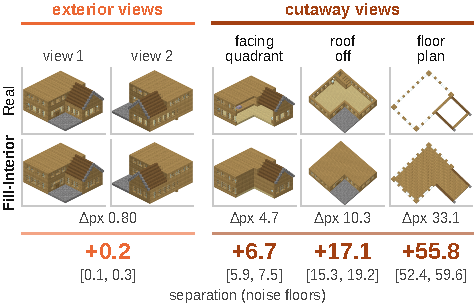
\includegraphics[width=\linewidth]{figures/fig9_cutaway}
\caption{\textbf{The same encoder and statistic, only the views changed.} Each pair is a
held-out build over its \solidify{} twin. \emph{Left:} two of the four exterior views the
standard protocol renders, visually indistinguishable for this build at a mean pixel difference
of $0.8/255$. \emph{Right:} three cutaway protocols on the same builds, each with its separation in
noise floors, with a paired-subsample $95\%$ interval. DINOv2-B,
unbiased KID, $n{=}256$ against $512$ reference builds; full ablation in
\supptab{tab:ablation}.}
\label{fig:cutaway}
\end{figure}

%TL;DR of paragraph: varying encoder, view budget, projection and pooling changes nothing.
The finding could indict DINOv2 at four views rather than render-and-embed as a class. It
does not (Figure~\ref{fig:cutaway}, \supptab{tab:ablation}). Four other encoders, CLIP
ViT-B/16 and B/32, ImageNet-supervised ResNet-50 and the Inception network FID itself uses,
land between $0.0$ and $0.2$ noise floors, as does our DINOv2-B. Eight and sixteen views
covering roof and underside read $+0.2$ and $+0.1$, perspective projection reads $+0.1$, and
face-on elevations, which look straight through windows, read $+4.4$ at $n{=}256$ (\suppsec{app:views25d}).

%TL;DR of paragraph: the cutaway rows are the positive control that makes this a statement about information rather than features.
The cutaway rows are the positive control. The same encoder and the same statistic recover
the interior at $6.7$ to $55.8$ noise floors once the view protocol stops hiding it, which
makes this a statement about \emph{information} rather than about features:
\textbf{the standard view protocol does not put interior structure into the image, so no
encoder downstream of it can score that structure.} A cutaway is not itself a good metric,
because a section view discards the facade the render tier exists to read.

%TL;DR of paragraph: under an opaque renderer the invisibility is exact, which makes it a theorem rather than a measurement.
Under an \emph{opaque} renderer interior damage provably never reaches the image: filling sealed air cannot alter any exterior
view, so no encoder and no statistic can separate it at any sample size. Rendered with
glass opaque, one fixed texture atlas and a CPU rasterizer, all $1{,}596$ test-split views are
bit-identical under both \solidify{} and \hollow{}, so their \mvkid{} separation from real is
exactly $0$; \suppsec{app:hull} gives the proof.

%TL;DR of paragraph: our renderer leaks through glass and an atlas artifact, the leak moves each build's feature in proportion, and the set statistic does not follow it.
Our default renderer is not opaque, and under it \solidify{} alters $\mathbf{91\%}$ of the
$1{,}596$ test-split views, touching a median $1.23\%$ of pixels at a median maximum
channel difference of $\mathbf{128/255}$. Doorways never leak, as air a doorway reaches is
not sealed; glass in front of a filled void does, as does an atlas artifact of our mesh
builder, and with the atlas fixed the fill shows in $67\%$ of houses (\suppsec{app:hull}).
Binned by how much of its silhouette the fill changes, each house's DINOv2 feature moves
in proportion (Spearman $0.96$), yet no bin moves \mvkid{} by more than $1.4$ noise floors:
the leak reaches single images, not the set statistic.

\subsection{Both Directions and Three Domains}
\label{sec:hollow}

%TL;DR of paragraph: hollowing is as invisible as filling, so the blindness runs along the whole interior axis, and separations compare within a run.
The corruption this field actually produces is the converse of \solidify{}: the hollow
shells that surface-fitted mesh and implicit generators emit. It is equally invisible. Against
the leaderboard's reference and noise floor at $n{=}256$, \mvkid{} places \hollow{} at $+0.04$
noise floors and \solidify{} at $+0.35$, while \vkid{} places the same two arms at $+265.4$
and $+444.36$ (\suppsec{app:views25d}). The render metric is blind along the whole interior
axis rather than to one hand-built probe.

%TL;DR of paragraph: the LEGO replication reproduces the qualitative structure, and a published LEGO generator separates on both tiers.
\label{sec:lego}The pattern is not a property of Minecraft houses. On the LEGO corpus
(Table~\ref{tab:lego}, \suppfig{fig:lego}), \mvkid{} places the solidified arm
\emph{below} the real floor and \vkid{} at $\mathbf{+118.6}$, while the render metric
separates \matshuffle{} at $+140.0$ and \monochrome{} at $+685.8$. A published LEGO
generator, BrickGPT \citep{pun2025brickgpt}, prompted with captions of $253$ held-out test
objects, separates on both tiers, $+11.8$ and $+51.5$, beside a solidified control at
$-0.09$ and $+36.4$; its own validity and stability reproduce (\suppsec{app:brickgpt}).

\begin{table}[t]
\centering
\small
\setlength{\tabcolsep}{4pt}
\caption{\textbf{LEGO.} Separation from held-out real in each run's own noise floors.}
\label{tab:lego}
\begin{tabular}{lrr}
\toprule
arm & \mvkid{} & \vkid{} \\
\midrule
\multicolumn{3}{l}{\emph{ShapeNet bricks with a sealed void, $n{=}256$}} \\
\solidify{}    & $\mathbf{-0.01}$ & $\mathbf{+118.6}$ \\
\matshuffle{}  & $+140.0$ & $+0.0$ \\
\monochrome{}  & $+685.8$ & $+0.0$ \\
\midrule
\multicolumn{3}{l}{\emph{StableText2Brick test split, $n{=}253$}} \\
\solidify{}    & $-0.09$ & $+36.4$ \\
BrickGPT \citep{pun2025brickgpt} & $+11.8$ & $+51.5$ \\
\bottomrule
\end{tabular}
\end{table}

%TL;DR of paragraph: the third domain, Objaverse meshes, shows the same split between exterior and interior observation.
On $290$ multi-room Objaverse buildings, the third domain, a DINOv2 kernel distance on four
exterior views reads $+0.0$ for both removing the hidden faces and filling the hidden volume,
at both seeds, while four cutaway views read $9.0$ to $13.7$ and \vkid{} $23.7$ to $118.4$
(\supptab{tab:probe3d}).

\subsection{Complementary Blindness and the Leaderboard}
\label{sec:complementary}

\begin{table*}[t]
\centering
\small
\setlength{\tabcolsep}{3pt}
\caption{\textbf{The leaderboard} ($n{=}256$ per arm, $399$ reference builds). Appearance
and geometry are null-standardized $z$-scores: the arm's distance from held-out real over
the standard deviation of $48$ real-vs-reference draws at this $n$. That deviation shrinks by
a factor of $0.49$ to $0.72$ when $n$ doubles, so the $z$-scores are \textbf{not comparable across $n$}; the raw
MMD$^2$ columns ($\times 10^3$) are stable in $n$. \blockscore{} is the
\textbf{maximum} across five pillars; palette and the two structure pillars never determine
it here, and the structure pillars use a coarser in-run scale (\suppsec{app:blockscore}). Rank is the $95\%$ interval over $1{,}000$ subsample
replicates; an interval spanning several places marks a tie. $\dagger$~marks the contaminated
checkpoint of \suppfig{fig:contamination}, unrankable and shown for comparison. ``Twins'' is
the within-set near-twin rate, the share of builds with a near-copy elsewhere in the same
set ($0.8\%$ for held-out real); its gate disqualifies four rows, whose pillars are shown
for comparison.}
\label{tab:leaderboard}
\begin{tabular}{rlrlrrrr}
\toprule
& & & & \multicolumn{2}{c}{$z$ (noise floors)} & \multicolumn{2}{c}{raw MMD$^2$} \\
\cmidrule(lr){5-6}\cmidrule(lr){7-8}
rank & arm & \blockscore{}~$\downarrow$ & worst pillar & appearance & geometry & \mvkid{} & \vkid{} \\
\midrule
1 & \realheld{} \emph{(anchor)}      & $0.00$   & ---        & $+0.00$   & $+0.00$ & $0.001$ & $-0.14$ \\
\midrule
\multicolumn{8}{l}{\emph{submissions}} \\
$(2)^\dagger$ & \voxar{} \emph{(contaminated)} & $229.29$ & geometry & $+128.87$ & $+229.29$ & $0.208$ & $12.08$ \\
3 & \voxar{} \emph{(clean)}          & $285.22$ & geometry   & $+157.40$ & $+285.22$ & $0.254$ & $15.06$ \\
4 & \voxarun{} \emph{(clean)}        & $345.10$ & geometry   & $+182.86$ & $+345.10$ & $0.295$ & $18.25$ \\
5--7 & \patchstitch{}                & $431.70$ & appearance & $+431.70$ & $+368.21$ & $0.696$ & $19.48$ \\
10 & \randomvox{}                    & $1087.06$ & appearance & $+1087.06$ & $+727.48$ & $1.752$ & $38.63$ \\
\midrule
\multicolumn{8}{l}{\emph{probes and controls: known damage, not submissions}} \\
5--7 & \textbf{\solidify{}}          & $444.36$ & geometry   & $\mathbf{+0.35}$ & $\mathbf{+444.36}$ & $0.001$ & $23.54$ \\
5--7 & \matshuffle{}                 & $422.43$ & appearance & $+422.43$ & $\mathbf{+0.00}$ & $0.681$ & $-0.14$ \\
8 & \monochrome{}                    & $535.36$ & appearance & $+535.36$ & $+0.00$ & $0.863$ & $-0.14$ \\
9 & \copynoise{}                & $619.13$ & geometry   & $+271.94$ & $+619.13$ & $0.439$ & $32.86$ \\
\midrule
\multicolumn{8}{l}{\emph{disqualified: refused a rank, with the reason}} \\
  & Dream-Cubed \citep{merino2026dreamcubed} & DQ & twins $59.8\%$ & $+165.71$ & $+146.64$ & $0.268$ & $7.67$ \\
  & \emph{vanilla village templates} ($n{=}174$) & DQ & twins $67.2\%$ & $+110.21$ & $+202.95$ & $0.178$ & $10.67$ \\
  & \gabled{}                       & DQ & twins $20.7\%$ & $+535.62$ & $+620.98$ & $0.863$ & $32.96$ \\
  & \hollowbox{}                    & DQ & twins $24.6\%$ & $+864.00$ & $+645.86$ & $1.392$ & $34.28$ \\
  & \singlemode{}                    & DQ & \multicolumn{5}{l}{mode collapse, $+44.9$ spreads on voxel diversity} \\
  & \traincopy{}                     & DQ & \multicolumn{5}{l}{memorization, $+10.1$ spreads on retrieval percentile} \\
  & Dream-Cubed \emph{(whole chunk)} & DQ & \multicolumn{5}{l}{mode collapse, $+24.0$ spreads on voxel diversity: every chunk is a slab of terrain} \\
\bottomrule
\end{tabular}
\end{table*}

%TL;DR of paragraph: each tier is fooled by the corruption aimed at it and rescued by the other, and the asymmetry between the two failures is large.
Table~\ref{tab:leaderboard} shows the complementarity directly. \solidify{} reads $+0.35$
on appearance against $+444.36$ on geometry, and \matshuffle{} is the converse, $+422.43$
on appearance against \emph{exactly} $+0.00$ on geometry. Noise floors grow with $n$, so
we compare tiers by effect size, $\sqrt{\text{MMD}^2}$ as a fraction of \randomvox{}'s
under the same metric: \solidify{} sits at $0.03$ on appearance, inside the $0.03$ that
fresh real draws reach, and at $0.78$ on geometry (\suppsec{app:failrate}). Each tier is fooled by the corruption aimed at it and
rescued by the other, which is why \blockscore{} takes the worst pillar. The two failures
differ in severity: the best attack we have on \vkid{}, \patchstitch{}, buys
near-perfect local occupancy statistics with globally incoherent structure and still sits
at an effect size of $0.71$ on geometry. The two feature spaces dissociate build by build as well: asked for each probe's
nearest held-out real build, the render features return a filled house's own source
$100\%$ of the time and \vkid{}'s features $26\%$, and for \matshuffle{} the proportions
reverse, $26\%$ against $100\%$ (\suppfig{fig:nn}).

%TL;DR of paragraph: the published generator is disqualified for repeating itself, which a new within-set gate catches and the train-split gates did not.
Dream-Cubed \citep{merino2026dreamcubed}, the one published generator we score, is
disqualified (\suppsec{app:dreamcubed}). Scored on the largest constructed component of
each terrain chunk its village checkpoint emits, its builds copy nothing from our training
split (duplicate rate $0.004$) but copy each other: $59.8\%$ have a near-copy in the same
set (occupancy IoU $\geq 0.8$ under rotation, mirroring and translation), against $0.8\%$
for held-out real, and they are vanilla village pieces, $36\%$ of them roofless
enclosures. Neither novelty gate saw this, so we added a within-set near-twin gate under
the duplicate gate's rule. It disqualifies Dream-Cubed at $+29.5$ spreads, the two
parametric baselines, and the game's own village templates, which would otherwise score
$202.95$, ahead of every model we trained.

%TL;DR of paragraph: the geometric separation does not come from the added mass or from the sealed-interior scalar.
Deleting \vkid{}'s size term and sealed-interior scalar leaves $197.3$ of its $201.8$
floors on \solidify{} in the protocol run (\suppsec{app:descriptor}). Every leave-one-family-out variant, every random half of its
dimensions and descriptors with no hand design (random 3D CNNs, raw $3^3$ patterns) pass
all gates, the last at $257$ to $437$ floors on \solidify{} (\suppsec{app:vkid-robust}).

%TL;DR of paragraph: a mass-matched control separates on the render metric and not the geometric one, which is the dissociation stated without a probe-specific argument.
The sharper test is a control matched on the quantity in question. \growshell{} dilates the
solid outward until it has added \emph{exactly} the number of blocks \solidify{} adds to
that build, which it achieves to within one block on $128$ of $128$ builds at a median of
$196$. Same builds, same material, same mass, and the only difference is whether the new
mass goes inside or outside. The two metrics then part company completely. In that run
\mvkid{} places \growshell{} at $\mathbf{+102.3}$ noise floors and \solidify{} at
$\mathbf{+0.3}$, while \vkid{} places them at $214.5$ and $201.8$. No block count could
produce that pair of rows.

%TL;DR of paragraph: a required provenance field caught contamination that no statistic saw, and the maximum rule names a different failure for each learned arm.
The $\dagger$ row is our own autoregressive checkpoint, which had trained on $346$ of the
$399$ test builds ($87\%$). No distribution statistic and no memorization gate saw it, at a
duplicate rate of $0.000$; a required split declaration did, and retrained on the clean
split the arm loses its margin over the language-model baselines (\suppsec{app:casestudy}).
Benchmarks in this domain should require that declaration and refuse to rank arms that
cannot make it. The maximum rule also names a different failure for each learned arm: the
clean \voxar{} is geometry-limited, $+285.22$ against $+157.40$ on appearance, and
\patchstitch{} is limited by appearance, so a mean over pillars would hide both.

\subsection{Limitations}
\label{sec:limitations}

%TL;DR of paragraph: what each tier measures, stated as scope: the proof covers opaque rendering, V-KID reads local geometry, and neither tier scores interior appearance.
The invisibility is a theorem about opaque rendering (\suppsec{app:hull}); for translucent
renderers it is a measured attenuation, here on one renderer, and a path tracer sharing no
code with ours is the natural replication. \vkid{} reads local geometry. Global coherence is
a separate axis, which \patchstitch{}, assembled from patches of real builds, exposes by
scoring closer to real than the simple but coherent \gabled{} on both tiers, so it stays a
standing control (\suppsec{app:vkid-robust}). \vkid{} is blind to materials by construction,
and neither tier scores how an interior \emph{looks}: cross-section views see it but rank
arms by texture (\suppsec{app:views25d}), so interior appearance is an open measurement.
Detecting interior change is not ranking interior function: \vkid{} accepts cluttered
interiors, and a walk-through test sides with \mvkid{} on $33$ of $40$ reversed generator pairs (\suppsec{app:functional}).

%TL;DR of paragraph: the noise-floor unit depends on n, and the one published Minecraft generator needs an extraction step.
A noise floor is a run's own statistic and roughly halves when $n$ doubles, so magnitudes
compare within a run ($n{=}256$ for the leaderboard, $128$ elsewhere) and only ranks and
ratios carry across runs (\suppsec{app:nscale}). The generator released with this
corpus \citep{chen2019voxelcnn} reports a cumulative chamfer distance,
which is exactly invariant to our probe (\S\ref{sec:related}).

\section{Conclusion}

%TL;DR of paragraph: what we found: the inherited render-and-embed protocol measures a structure's surface, so interior damage passes it untouched.
Evaluation for {3D} structure generation was inherited from image generation, and the
inheritance carries a specific defect. Rendering a structure and embedding the renders
measures its surface, and a building is not its surface. Filling every interior in a corpus
of real buildings is invisible to a multi-view kernel distance that resolves every
corruption reaching the exterior. That invisibility survives every encoder, view
budget and statistic we try, point-cloud metrics on visible surfaces and an image judge,
and a cutaway view removes it: what the render metric misses is not the quantity of the
change but its location.

%TL;DR of paragraph: the general lesson, that a metric inherits the blind spots of the observation it is built on, and what follows for practice.
A metric therefore earns the right to rank models by first resolving damage of known
severity. The price is a handful of corruption arms scored beside the real reference in
every run, and what it buys is that a result resting on a blind metric fails in the lab
rather than in the literature. Structure that decides whether a generated
object is usable, and that no camera can photograph, has to be measured directly,\label{endofmain} and the
same audit is owed to mesh and implicit {3D} generation.


% ---- end of the 8-page main text (label endofmain is in 7_conclusion) ----
% LLM Usage Statement: mandatory, excluded from the page limit, placed after the
% main text and before the references.
% ---------------------------------------------------------------------------
% CVPR 2027 requires an LLM Usage Statement (desk reject if missing). It does
% NOT count against the 8-page limit; it sits after the main text and before
% the references. It must be truthful: it is the authors' attestation.
% Keep this accurate as the paper changes.
% ---------------------------------------------------------------------------
\section*{LLM Usage Statement}

%TL;DR of paragraph: we disclose AI assistance by dividing the labor rather than with a blanket statement.
We used a generative AI coding assistant substantially in preparing this work,
and describe the division of labor rather than a blanket disclosure.

%TL;DR of paragraph: the assistant drafted text, figure code, parts of the suite and the literature search.
\textbf{Where it was used.} Drafting and editing the text of this paper;
implementing the figure-generation code; implementing parts of the evaluation
suite and the probes; and conducting literature
searches, including the prior-art check that identified
\citet{binkowski2018kid}'s Appendix~B.2 as the source of the mixture identity in
\suppsec{app:failrate} and the limitation already stated by
\citet{merino2026dreamcubed}.

%TL;DR of paragraph: the research questions, design and interpretation are the authors', and no number came from a language model.
\textbf{Where it was not.} The research questions, the experimental design, the
decision of what to measure, and the interpretation of results are the authors'.
No experimental result, numerical value or table entry in this paper was
produced by a language model: every number is emitted by the released code from
a recorded run, and the figures read those runs directly rather than
transcribing them.

%TL;DR of paragraph: citations and arithmetic were checked, which found and fixed several errors.
\textbf{Verification.} Every citation was checked against arXiv or the official
proceedings, and every numeral in the paper is re-derived from a recorded run by a
registered check in the released code. The authors take full responsibility for the
contents of the paper, including any remaining errors.


{
    \small
    \bibliographystyle{ieeenat_fullname}
    \bibliography{references,references_new}
}

% Supplementary material is a separate PDF: see supp.tex.

\end{document}
